\chapter{Progettazione concettuale}

    
    \section{Schema Concettuale}
        \begin{flushleft}
            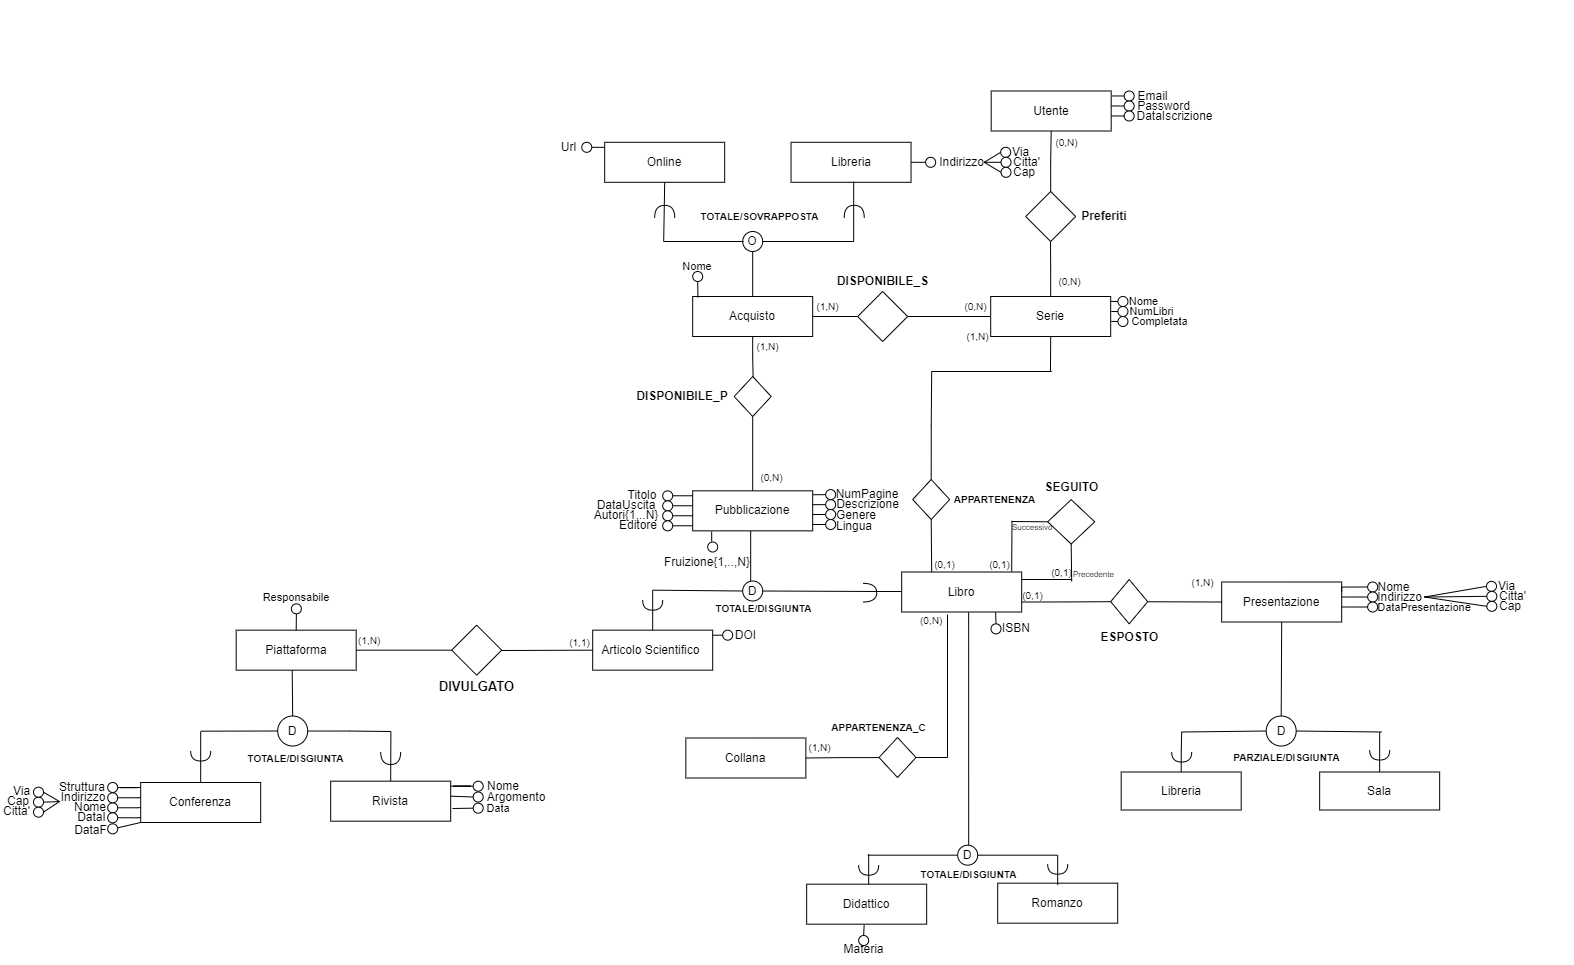
\includegraphics[width=0.98\textwidth]{Immagini/DiagrammaErNonRistrutturato.png}
        \end{flushleft}
\newpage
    \section{Dizionario delle entità e delle associazioni}
\begin{center}    
    \begin{tabular}{ | m{5cm} | m{5cm}| m{6cm} | } 
        \hline
             {\bf Entità} & {\bf Descrizione}  & {\bf Attributi: descrizione}\\ 
         \hline
               Pubblicazione & Rappresentazione generale delle pubblicazioni, entità padre di "Articolo Scientifico" e "Libro".   
                &  
                 {\bf Titolo:} Rappresenta il titolo della pubblicazione.\par 
                 {\bf DataUscita:} Indica l'anno di uscita della pubblicazione.\par 
                 {\bf Autori[1..n]:} Attributo multiplo che rappresenta gli autori.\par 
                 {\bf Editore:} Rappresenta il nome dell'editoria.\par 
                 {\bf NumPagine:} Indica il numero delle pagine della pubblicazione.\par 
                 {\bf Descrizione:} Definisce la descrizione posta dall'autore.\par 
                 {\bf Genere:} Rappresenta il genere della pubblicazione.\par 
                 {\bf Lingua:} Indica in che lingua è scritta la pubblicazione.\par 
                 {\bf Fruizione[ Cartaceo, Digitale, AudioLibro]:} Attributo multiplo che definisce la modalità con la quale può essere fruito.\par 
             \\
         \hline
          \end{tabular}
          \begin{tabular}{ | m{5cm} | m{5cm}| m{6cm} | } 
            \hline
            Libro & Rappresentazione specifica di una pubblicazione, che traccia i libri, entità figlia dell'entità Pubblicazione e entità padre delle entità "Romanzo" e "Didattico".
            &    
            {\bf ISBN:} Identificativo del libro.\par 
            \\
             \hline

            Articolo Scientifico & Rappresentazione specifica di una pubblicazione che traccia gli Articoli Scientifici, entità figlia dell'entità "Pubblicazione".
            &  
             {\bf DOI:} Identificatore dell'articolo scientifico.\par 
             \\ 
        \hline
            Didattici & Rappresenta la specializzazione dell'entità "Libro" composta dai libri didattici che hanno come attributo distintivo la materia.
            & 
            {\bf Materia:} Indica la materia del libro didattico.
            \par 
            \\ 
             \hline
       
        
            Romanzo & Rappresentazione della specializzazione dell'entità "Libro" che contiene i Romanzi & \\ 
        \hline
            Collana & Rappresenta l'insieme di libri con una caratteristica comune & \\ 
        \hline

      \end{tabular}
          \begin{tabular}{ | m{5cm} | m{5cm}| m{6cm} | }  
        \hline


            Piattaforma & Rappresentazione generale delle piattaforme dove vengono  pubblicati gli articoli scientifici, entità padre di "Conferenza" e "Rivista". 
            & {\bf Responsabile:} Rappresenta il coordinatore della piattaforma.\par \\ 
        \hline

        
            Conferenza & Specializzazione di "Piattaforma", entità figlio che traccia le conferenze
            & {\bf Struttura:} Indica il luogo in cui si è svolta o si svolgerà la conferenza.\par
              {\bf  Indirizzo{\large[Via,Città,CAP]:}}  Definisce la locazione della struttura\par
              {\bf Nome:} Rappresenta il nome della struttura\par
              {\bf DataI:} Indica la data in cui inizia l'evento\par
              {\bf DataF:} Indica la data in cui finisce l'evento\par
              \\ 
              \hline
              
      

        
             Rivista & Specializzazione di "Piattaforma", entità figlio che traccia le riviste
             & {\bf Nome:} Delinea il nome della rivista\par
               {\bf Argomento:} Definisce l'argomento della rivista \par
               {\bf Data:} Indica la data in cui è stata pubblicata la rivista\par
                \\ 
        \hline
        \end{tabular}
       \begin{tabular}{ | m{5cm} | m{5cm}| m{6cm} | }   
       \hline
             Presentazione & Rappresentazione generale delle Presentazioni dove vengono pubblicati i libri, entità padre di "Libreria" e "sala".
             & 
             {\bf Nome:} Raffigura il nome della presentazione.\par 
             {\bf  Indirizzo{\large[Via,Città,CAP]:}} Indica il luogo dove si terra la presentazione.\par 
             {\bf DataPresentazione :} Definisce il luogo della presentazione.\par 
             \\ 
        \hline
             Libreria & Specializzazione di "Presentazione", entità figlio che traccia le librerie. & \\ 
        \hline
             Sala & Specializzazione di "Presentazione", entità figlio che traccia le sale. & \\ 
       \hline

             Serie & Raccolta di libri facente parte della stessa sequenza & 
             {\bf Nome:} Indica il nome della serie.\par
             {\bf NumLibri:} Rappresenta il numero dei libri della serie.\par
             {\bf Completata:} Identifica se la serie è completa o meno.\par\\ 
        \hline
             Acquisto & Entità generale che indica dove è possibile acquistare una pubblicazione, entità padre dell'entità "Online" e "libreria". 
             & 
             {\bf Nome:} Definisce il nome della libreria \par 
             \\ 
            \hline
             \end{tabular}
       \begin{tabular}{ | m{5cm} | m{5cm}| m{6cm} | }   
       \hline
             Online & Specializzazione dell'entità "Acquisto" che rappresenta i siti web dove potere acquistare i libri
             & {\bf URL:} Indica l'indirizzo web del sito.\par\\ 
        \hline
             Libreria & Specializzazione dell'entità "Acquisto" che rappresenta le librerie fisiche dove potere acquistare i libri.
             & 
             {\bf  Indirizzo{\large[Via,Città,CAP]:}} Attributo composto, indica la posizione della libreria fisica.\par 
             \\ 
        \hline
             Utente & Rappresenta gli utenti che accederanno al database.
             & {\bf Email:} Identificativo dell'utente.\par
                {\bf Password:} Indica la password del profilo utente.\par
                {\bf DataIscrizione:} Rappresenta la data d'iscrizione dell'utente.\par\\ 
        \hline
    \end{tabular}


\begin{tabular}{ | m{5cm} | m{5cm}| m{6cm} | } 
        \hline
             {\bf Associazione} & {\bf Descrizione}  & {\bf Regole di lettura} \\ 
         \hline
           Divulgato &  Associazione 1 a N tra "Piattaforma" e "Articolo scientifico", indica la piattaforma dove l'articolo scientifico è stato pubblicato.  &  Una "Piattaforma" deve pubblicare uno o più "Articoli scientifici",  un "Articolo scientifico" deve essere pubblicato da una e una sola "Piattaforma".\\ 
         \hline
          Esposto &  Associazione 1 a N tra "Presentazione" e "Libro", indica il luogo in cui un libro è stato presentato.  &   Una "Presentazione" deve esporre uno o più "Libri", Un "Libro" può essere esposto in nessuna o una  "Presentazione".\\ 
         \hline
          Seguito &  Associazione ricorsiva 1 a 1 tra "Libro" e "Libro", esprime il concetto di successione di libri in una serie.  &   Un "Libro" può essere il successivo di nessuno o un "Libro" e un "Libro" può essere precedente di nessuno o un "Libro".\\ 
         \hline
          Appartenenza  &  Associazione 1 a N tra "Serie" e "Libro", rappresenta l'appartenenza di un libro in una serie. &   Una "Serie" deve avere uno o più "Libri", un "Libro" può appartenere a nessuna o una "Serie".\\ 
       \hline
          Preferiti &  Associazione N a N tra "Utente" e "Serie", utilizzata per rappresentare le preferenze di un utente. & Un "Utente" può avere preferita nessuna o più "Serie", una "Serie" può essere preferita da nessuno o più "Utenti".\\
       \hline
         Disponibile\_S  &  Associazione N a N tra "Serie" e "Acquisto", indica la possibilità di una serie di essere acquistata e dove.  &  Una "Serie" può essere disponibile in nessuno o più "Acquisti", un "Acquisto" può avere disponibile nessuna o più "Serie".\\ 
         \hline 
\end{tabular}



    

\begin{tabular}{ | m{5cm} | m{5cm}| m{6cm} | }  
       \hline
         Disponibile\_P  &  Associazione N a N tra "Pubblicazione" e "Acquisto".  & Una "Pubblicazione" può essere disponibile in nessuno o più "Acquisti", un "Acquisto" può avere disponibile nessuna o più "Pubblicazioni".\\ 
         \hline
         
       
       Appartenenza\_C  &  Associazione N a N tra "Collana" e "Libro". & Una "Collana" deve possedere uno o più "Libri", un "Libro" può appartenere a  nessuna o più "Collane".\\ 
       \hline
 \end{tabular}
\end{center}